
This document presents the status of the New Small Wheel (NSW) Trigger Processor (TP) project and it is the main source of information for the ATLAS Design Review.
Information about the whole New Small Wheel detector system can be found in the New Small Wheel Technical Design Report\,\cite{NSWTDR}.
The Trigger Processor specifications are presented in Section\,\ref{sec:specs}.
These include a description of the interfaces to the two NSW trigger detectors (Micromegas, \MM, and small Thin Gap Chambers, \stgc),
of the interface to the muon end-cap Sector Logic and of the ancillary functionality of the Trigger Processor.
Section\,\ref{sec:algorithms} presents the trigger algorithms under consideration for both detector technologies,
including studies of the corresponding expected trigger performance and information regarding trigger duplicate handling.
The two options for the Trigger Processor hardware platforms are briefly introduced in Section~\ref{sec:hardware-platforms}, including a specification comparison and the criteria for a decision, with
further details provided in Refs.\,\cite{hardware-LAr-Carrier,hardware-LAr-OTC,hardware-SRS-Carrier,hardware-SRS-Mezz}.
The plans for testing the Trigger Processor hardware and firmware are presented in Section\,\ref{sec:testing},
followed by a brief discussion on the compatibility of the project with \PhaseTwo.
The document concludes with a concise overview of the project organization in Section\,\ref{sec:organization}.
%, including the schedule and responsibilities.
%Finally, the fiber plant is presented in Appendix~\ref{app:specs-fibers}.

\subsection{Overview of the NSW trigger}
\label{sec:Overview}

The main goal of the NSW trigger is to provide additional information to the muon Level-1 trigger (L1) in the \endcap region $1.0<|\eta|<2.4$, in order to dramatically reduce fake triggers arising from particles that are not high-\pt muons originating in the interaction point (IP).
A major source of fake triggers is low energy particles, mainly protons, generated in the material located between the Small Wheel and the end-cap middle station, the Big Wheel (BW).
As shown in Figure\,\ref{fig:NSW-Z}, these particles can cross the end-cap trigger chambers at an angle similar to that of real high \pt muons.
The NSW trigger signal is based on track segments produced online by the small Thin Gap Chambers (\stgc) and Micromegas chambers (\MM) comprising the NSW detectors.
These candidate track segments are input to the new Sector Logic (SL) that uses the information to corroborate trigger candidates from the BW TGC chambers.
The sector logic sends Level-1 trigger candidates to the ATLAS Muon Central Trigger system.

\begin{figure}[htb]
  \centering
  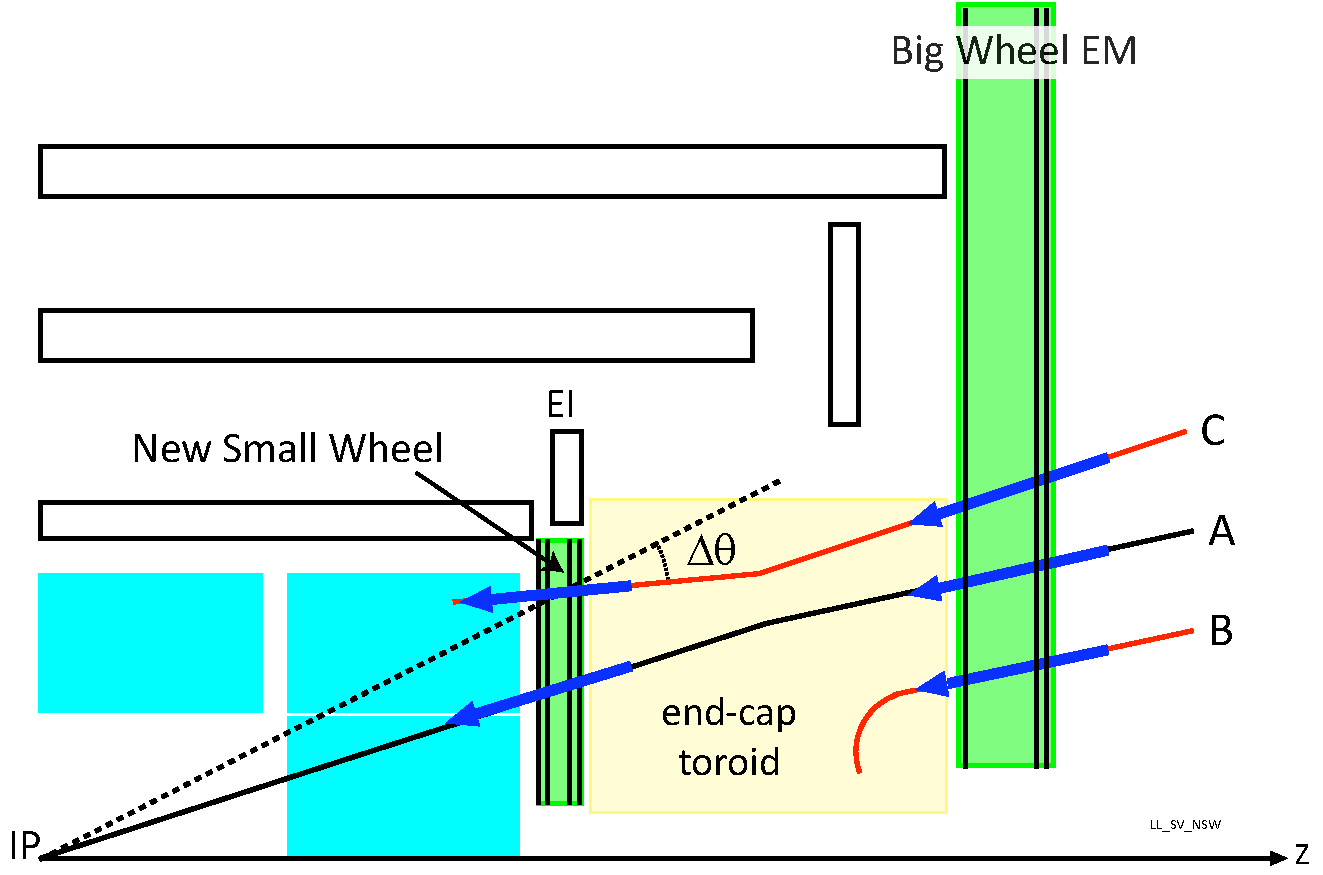
\includegraphics[width=0.6\textwidth]{figures/LL_SV_NSW.pdf}
%  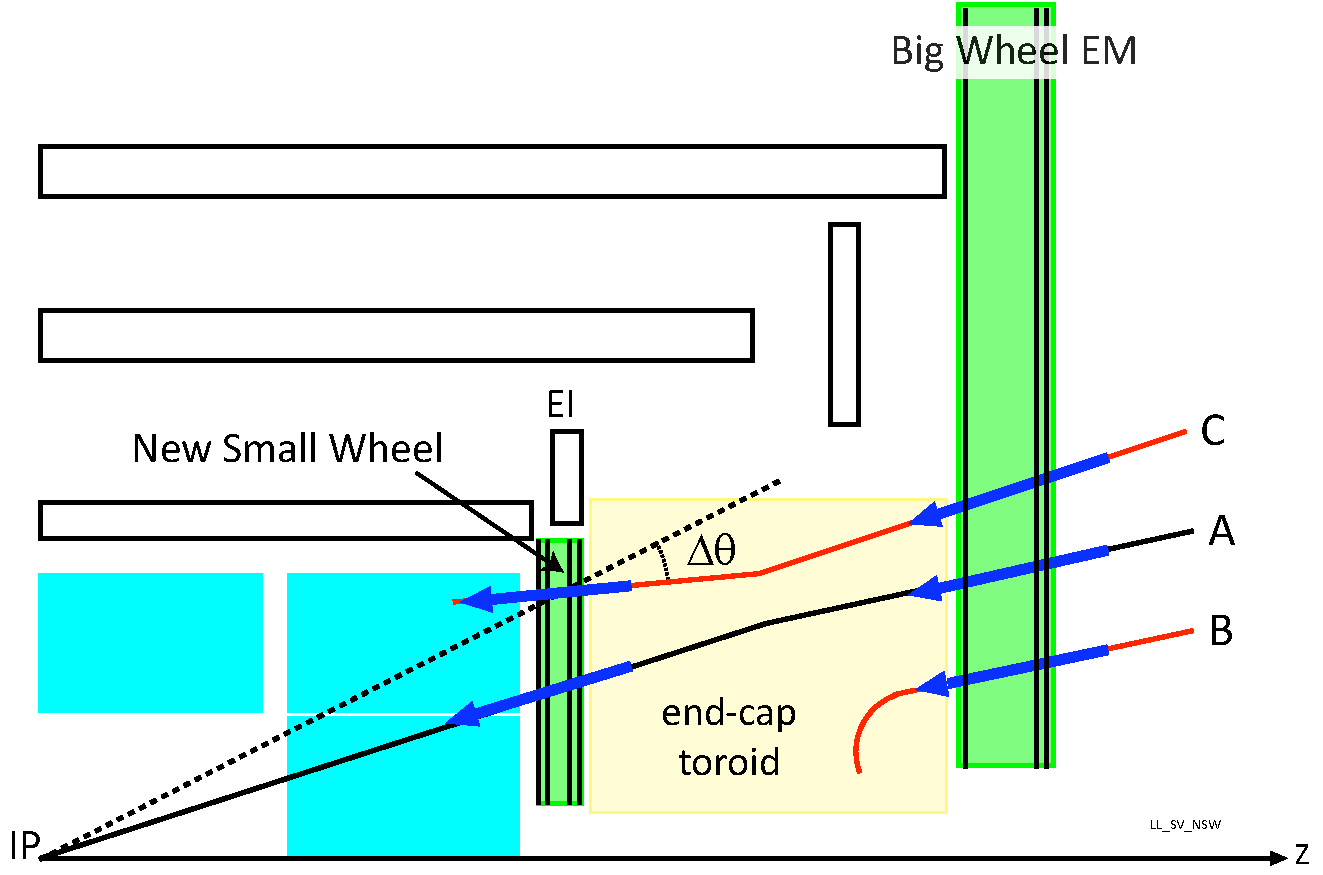
\includegraphics[trim=4cm 1.0cm 6.5cm 1.0cm, clip=true, width=0.6\textwidth]{figures/LL_SV_NSW.pdf}
  \caption{\small Schematic of the muon \endcap trigger. The existing Big Wheel trigger accepts all three tracks shown. With the addition of the NSW to the muon end-cap trigger, only track `A', the desired track, which is confirmed by both the Big Wheel and the NSW, will be accepted. Track `B' will be rejected because the NSW does not find a track coming from the interaction that matches the Big Wheel candidate. Track `C' will be rejected because the NSW track does not point to the interaction point (IP).
  The NSW logic restricts $\Delta\theta$ to a value consistent with the track to have originated from the IP.}
  \label{fig:NSW-Z}
\end{figure}

%\subsection{System layout and definitions}

\subsection{System granularity and terminology}
\label{sec:SystemLayout}

The \endcap trigger system operates independently on each detector \endcap (side A and side C).
Several other factors define the granularity of the \endcap trigger system.
The following recalls the terminology and boundary conditions of the overall \endcap trigger system:

\begin{itemize}
\item A {\bf New Small Wheel sector} comprises \sector of a wheel (i.e.\ one \endcap). Each wheel has eight large and eight small sectors. The detector and trigger sectors are coincidental.
\item The {\bf Big Wheel trigger detector} (BW-TGC) has 12 detector sectors per wheel.
Each sector is further divided into trigger sectors, four trigger sections per detector sector in the region at larger radius (\endcap region) and two trigger sectors in the region at smaller radius (forward region). This segmentation results in a total of 48 trigger sectors in the \endcap (larger radius) region and 24 trigger sectors in the forward region.
\item A {\bf Sector Logic board} serves two adjacent BW-TGC trigger sectors. For each side (A/C), there are 24 SL boards for the BW-TGC \endcap region and 12 SL boards for the BW-TGC forward region.
\item A SL board receives data from at most three NSW sectors.
\item For the NSW Trigger Processor, there is one {\bf FPGA} per detector technology (\MM or \stgc) per NSW sector. (\MM) and \stgc information is processed by separate algorithms in separate FPGAs. Depending on the hardware platform chosen, the two FPGAs will be located in the same mezzanine card (SRS option) or on two separate mezzanine cards (LAr option).
\item A {\bf NSW Trigger Processor ATCA board} (corresponding to two NSW sectors) contains the mezzanine cards (two or four depending on the hardware platform ultimately chosen) to serve a NSW octant.
\item One NSW trigger sector needs to deliver data to up to seven SL boards. The maximum fan-out of seven is needed for large NSW sectors, due to the overlap with the BW trigger sectors when multiple scattering, misalignments and magnetic field deformations are taken into account.
\end{itemize}


\subsection{Requirements and Limitations}
\label{sec:RequirementLimitations}

The main requirement for the NSW trigger is to provide track vector candidates from the NSW detectors to be matched to track segments from the BW.
The angular resolution on the NSW track vector candidates should be of 1\,mrad. In the data-taking period immediately after the installation of the NSW, during the Long Shutdown\,2 (LS2), the BW trigger granularity is limited to an angular resolution of 3\,mrad or larger. During the Long Shutdown\,3 (LS3), new BW trigger electronics and a new MDT Level-1 trigger will be deployed, allowing for 1\,mrad angular resolution in the BW.

\paragraph{Matching resolution requirements}
The NSW measures the radial coordinates in two planes, the azimuthal coordinate, $\phi$, and the angle, $\Delta\theta$, of track segments inside the wheel, i.e.\ before the end-cap toroid. $\Delta\theta$ is the angle of the segment with respect to an ‘infinite momentum track’, i.e.\ a line from the IP to the segment’s radial position in the NSW. The radial coordinate is measured by high-precision strips in both detectors. For the sTGC, $\phi$ is determined by the triggering tower of sTGC pads, and for the MM, by small angle stereo strips. The angle $\Delta\theta$ is to be measured to an accuracy close to 1\,mrad. The NSW trigger logic will rejects track segments with $\Delta\theta > \pm (7-15)$\,mrad (the final value will be determined from future studies).
The corroboration with the BW trigger is done by projecting the ‘infinite momentum track’ through the $R-\phi$ point of the segment in the NSW onto the BW’s $R-\phi$ array of Regions-of-Interest (RoI).
This matching requires the NSW trigger candidates to have:
\begin{itemize}\itemsep-6pt
\item $\phi$-resolution of 20\,mrad
\item $\eta$-resolution of 0.005
\end{itemize}
The angle $\Delta\theta$ is passed to the Sector Logic but is not used in the \PhaseOne trigger decision.

\paragraph{Simulation limitations}
The trigger model in the Athena simulation of both the sTGC and the MM trigger is not complete. A simulation of the correlated backgrounds is also needed. The following studies are particularly urgent:
\begin{itemize}\itemsep-4pt
\item Probability of finding track segments as a function of radius, in particular the probability for more than four candidates, in either \MM or \stgc, and for a total of eight candidates when duplicates are removed.
\item The $\phi$-resolution needed for matching to the BW RoI’s
\item Effects due to misalignment within the NSW and between the NSW and the BW
\end{itemize}


